\documentclass[border=6pt]{standalone}
\usepackage{tikz}
\usepackage[edges]{forest}
\usetikzlibrary{arrows.meta,positioning,calc,decorations.pathreplacing,shapes.geometric}
\begin{document}
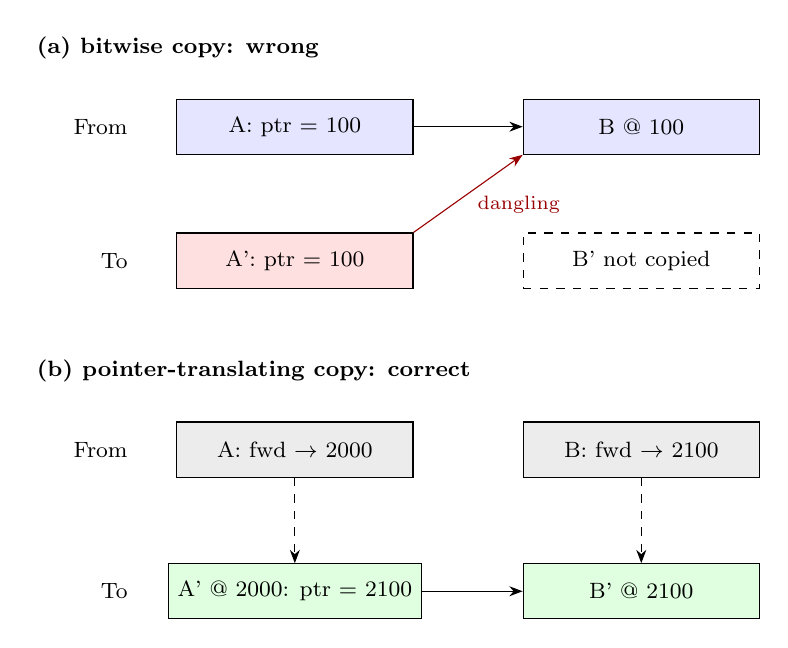
\begin{tikzpicture}[>=Stealth,font=\small,
 cell/.style={draw,minimum width=3.0cm,minimum height=0.7cm,align=center,font=\footnotesize}]
\node[font=\footnotesize\bfseries,anchor=west] at (-2.4,3.6) {(a) bitwise copy: wrong};
\node[font=\footnotesize,anchor=east] at (-1.0,2.6) {From};
\node[cell,fill=blue!10] (a1) at (1.0,2.6) {A: ptr $=$ 100};
\node[cell,fill=blue!10] (b1) at (5.4,2.6) {B @ 100};
\draw[->] (a1) -- (b1);
\node[font=\footnotesize,anchor=east] at (-1.0,0.9) {To};
\node[cell,fill=red!12] (a2) at (1.0,0.9) {A': ptr $=$ 100};
\node[cell,dashed] (b2) at (5.4,0.9) {B' not copied};
\draw[->,red!60!black] (a2.north east) -- node[below right,font=\scriptsize,pos=0.6,xshift=-4pt]{dangling} (b1.south west);
\node[font=\footnotesize\bfseries,anchor=west] at (-2.4,-0.5) {(b) pointer-translating copy: correct};
\node[font=\footnotesize,anchor=east] at (-1.0,-1.5) {From};
\node[cell,fill=gray!15] (a3) at (1.0,-1.5) {A: fwd $\to$ 2000};
\node[cell,fill=gray!15] (b3) at (5.4,-1.5) {B: fwd $\to$ 2100};
\node[font=\footnotesize,anchor=east] at (-1.0,-3.3) {To};
\node[cell,fill=green!12] (a4) at (1.0,-3.3) {A' @ 2000: ptr $=$ 2100};
\node[cell,fill=green!12] (b4) at (5.4,-3.3) {B' @ 2100};
\draw[->] (a4) -- (b4);
\draw[->,dashed] (a3) -- (a4); \draw[->,dashed] (b3) -- (b4);
\end{tikzpicture}
\end{document}
